\section{Результаты измерений}
\begin{table}[!ht]
    \centering
    \caption{Задание 7}
    \resizebox{\columnwidth}{!}{\begin{tabular}{|l|l|l|l|l|l|l|l|l|l|l|l|}
\hline
$C_n,\;\text{нФ}$ & $\nu,\;\text{КГц}$ & $U_C,\;\text{В}$ & $\mathcal{E},\;\text{В}$ & $Q$ & $R_{\Sigma},\;\text{Ом}$ & $I,\;\text{А}$ & $L,\;\text{мкГн}$ & $\rho,\;\text{Ом}$ & $R_{S_{max}},\;\text{Ом}$ & $R_L,\;\text{Ом}$ & $R_{S_{max}} / R_{\Sigma}$\\\hline
$24{,}8 \pm 0{,}05$ & $\left(32353{,}0 \pm 1{,}0\right)\cdot 10^{-3}$ & $2{,}57 \pm 0{,}08$ & $\left(100 \pm 3\right)\cdot 10^{-3}$ & $25{,}6 \pm 1{,}1$ & $7{,}8 \pm 0{,}3$ & $\left(129 \pm 4\right)\cdot 10^{-4}$ & $975{,}8 \pm 2{,}0$ & $198{,}4 \pm 0{,}4$ & $\left(1984 \pm 4\right)\cdot 10^{-4}$ & $7{,}6 \pm 0{,}3$ & $\left(25{,}6 \pm 1{,}1\right)\cdot 10^{-3}$\\\hline
$33{,}2 \pm 0{,}05$ & $\left(28010{,}0 \pm 1{,}0\right)\cdot 10^{-3}$ & $2{,}26 \pm 0{,}07$ & $\left(100 \pm 3\right)\cdot 10^{-3}$ & $22{,}6 \pm 1{,}0$ & $7{,}6 \pm 0{,}3$ & $\left(132 \pm 4\right)\cdot 10^{-4}$ & $972{,}5 \pm 1{,}5$ & $171{,}1 \pm 0{,}3$ & $\left(1711 \pm 3\right)\cdot 10^{-4}$ & $7{,}4 \pm 0{,}3$ & $\left(226 \pm 10\right)\cdot 10^{-4}$\\\hline
$47{,}6 \pm 0{,}05$ & $\left(23379{,}0 \pm 1{,}0\right)\cdot 10^{-3}$ & $1{,}95 \pm 0{,}06$ & $\left(100 \pm 3\right)\cdot 10^{-3}$ & $19{,}5 \pm 0{,}8$ & $7{,}3 \pm 0{,}3$ & $\left(136 \pm 4\right)\cdot 10^{-4}$ & $973{,}6 \pm 1{,}0$ & $143{,}02 \pm 0{,}15$ & $\left(1430{,}2 \pm 1{,}5\right)\cdot 10^{-4}$ & $7{,}2 \pm 0{,}3$ & $\left(195 \pm 8\right)\cdot 10^{-4}$\\\hline
$57{,}5 \pm 0{,}05$ & $\left(21352{,}0 \pm 1{,}0\right)\cdot 10^{-3}$ & $1{,}78 \pm 0{,}05$ & $\left(100 \pm 3\right)\cdot 10^{-3}$ & $17{,}8 \pm 0{,}8$ & $7{,}3 \pm 0{,}3$ & $\left(137 \pm 4\right)\cdot 10^{-4}$ & $966{,}3 \pm 0{,}8$ & $129{,}63 \pm 0{,}11$ & $\left(1296{,}3 \pm 1{,}1\right)\cdot 10^{-4}$ & $7{,}2 \pm 0{,}3$ & $\left(178 \pm 8\right)\cdot 10^{-4}$\\\hline
$68{,}0 \pm 0{,}05$ & $\left(19502{,}0 \pm 1{,}0\right)\cdot 10^{-3}$ & $1{,}67 \pm 0{,}05$ & $\left(100 \pm 3\right)\cdot 10^{-3}$ & $16{,}7 \pm 0{,}7$ & $7{,}2 \pm 0{,}3$ & $\left(139 \pm 4\right)\cdot 10^{-4}$ & $979{,}4 \pm 0{,}7$ & $120{,}01 \pm 0{,}09$ & $\left(12001 \pm 9\right)\cdot 10^{-5}$ & $7{,}0 \pm 0{,}3$ & $\left(167 \pm 7\right)\cdot 10^{-4}$\\\hline
$102{,}8 \pm 0{,}05$ & $\left(15939{,}0 \pm 1{,}0\right)\cdot 10^{-3}$ & $1{,}39 \pm 0{,}04$ & $\left(100 \pm 3\right)\cdot 10^{-3}$ & $13{,}9 \pm 0{,}6$ & $7{,}0 \pm 0{,}3$ & $\left(143 \pm 4\right)\cdot 10^{-4}$ & $969{,}9 \pm 0{,}5$ & $97{,}13 \pm 0{,}05$ & $\left(9713 \pm 5\right)\cdot 10^{-5}$ & $6{,}9 \pm 0{,}3$ & $\left(139 \pm 6\right)\cdot 10^{-4}$\\\hline
\end{tabular}
}
\end{table}
\[
    \left<L\right> = 973 \pm 4\;\text{мкГн}
\]
\[
    \left<R_{L}\right> = 7{,}2 \pm 0{,}2\;\text{Ом}
\]

\[
    R_{S_{max}} / R_{ \Sigma} \approx 0{,}02
\]

Погрешности приборов примерно равны погрешностям средних. Поэтому их влияние значительно.

\begin{table}[!ht]
    \centering
    \caption{АЧХ1}
    \begin{tabular}{|l|l|l|}
\hline
$C,\;\text{нФ}$ & $\nu,\;\text{КГц}$ & $U_C,\;\text{В}$\\\hline
$24{,}8 \pm 0{,}05$ & $\left(31568{,}0 \pm 1{,}0\right)\cdot 10^{-3}$ & $1{,}52 \pm 0{,}05$\\\hline
$24{,}8 \pm 0{,}05$ & $\left(31811{,}0 \pm 1{,}0\right)\cdot 10^{-3}$ & $1{,}9 \pm 0{,}06$\\\hline
$24{,}8 \pm 0{,}05$ & $\left(32014{,}0 \pm 1{,}0\right)\cdot 10^{-3}$ & $2{,}25 \pm 0{,}07$\\\hline
$24{,}8 \pm 0{,}05$ & $\left(32265{,}0 \pm 1{,}0\right)\cdot 10^{-3}$ & $2{,}54 \pm 0{,}08$\\\hline
$24{,}8 \pm 0{,}05$ & $\left(32110{,}0 \pm 1{,}0\right)\cdot 10^{-3}$ & $2{,}4 \pm 0{,}07$\\\hline
$24{,}8 \pm 0{,}05$ & $\left(31689{,}0 \pm 1{,}0\right)\cdot 10^{-3}$ & $1{,}71 \pm 0{,}05$\\\hline
$24{,}8 \pm 0{,}05$ & $\left(31866{,}0 \pm 1{,}0\right)\cdot 10^{-3}$ & $1{,}99 \pm 0{,}06$\\\hline
$24{,}8 \pm 0{,}05$ & $\left(31878{,}0 \pm 1{,}0\right)\cdot 10^{-3}$ & $2{,}02 \pm 0{,}06$\\\hline
$24{,}8 \pm 0{,}05$ & $\left(33214{,}0 \pm 1{,}0\right)\cdot 10^{-3}$ & $1{,}55 \pm 0{,}05$\\\hline
$24{,}8 \pm 0{,}05$ & $\left(33043{,}0 \pm 1{,}0\right)\cdot 10^{-3}$ & $1{,}76 \pm 0{,}05$\\\hline
$24{,}8 \pm 0{,}05$ & $\left(32749{,}0 \pm 1{,}0\right)\cdot 10^{-3}$ & $2{,}17 \pm 0{,}07$\\\hline
$24{,}8 \pm 0{,}05$ & $\left(32479{,}0 \pm 1{,}0\right)\cdot 10^{-3}$ & $2{,}49 \pm 0{,}07$\\\hline
$24{,}8 \pm 0{,}05$ & $\left(32579{,}0 \pm 1{,}0\right)\cdot 10^{-3}$ & $2{,}39 \pm 0{,}07$\\\hline
$24{,}8 \pm 0{,}05$ & $\left(32884{,}0 \pm 1{,}0\right)\cdot 10^{-3}$ & $1{,}98 \pm 0{,}06$\\\hline
$24{,}8 \pm 0{,}05$ & $\left(32622{,}0 \pm 1{,}0\right)\cdot 10^{-3}$ & $2{,}34 \pm 0{,}07$\\\hline
$24{,}8 \pm 0{,}05$ & $\left(33127{,}0 \pm 1{,}0\right)\cdot 10^{-3}$ & $1{,}66 \pm 0{,}05$\\\hline
\end{tabular}

\end{table}

\begin{table}[!ht]
    \centering
    \caption{АЧХ2}
    \begin{tabular}{|l|l|l|}
\hline
$C,\;\text{нФ}$ & $\nu,\;\text{КГц}$ & $U_C,\;\text{В}$\\\hline
$33{,}20 \pm 0{,}05$ & $\left(27101{,}0 \pm 1{,}0\right)\cdot 10^{-3}$ & $1{,}27 \pm 0{,}04$\\\hline
$33{,}20 \pm 0{,}05$ & $\left(27243{,}0 \pm 1{,}0\right)\cdot 10^{-3}$ & $1{,}43 \pm 0{,}04$\\\hline
$33{,}20 \pm 0{,}05$ & $\left(27678{,}0 \pm 1{,}0\right)\cdot 10^{-3}$ & $2{,}07 \pm 0{,}06$\\\hline
$33{,}20 \pm 0{,}05$ & $\left(27430{,}0 \pm 1{,}0\right)\cdot 10^{-3}$ & $1{,}69 \pm 0{,}05$\\\hline
$33{,}20 \pm 0{,}05$ & $\left(27782{,}0 \pm 1{,}0\right)\cdot 10^{-3}$ & $2{,}19 \pm 0{,}07$\\\hline
$33{,}20 \pm 0{,}05$ & $\left(27522{,}0 \pm 1{,}0\right)\cdot 10^{-3}$ & $1{,}83 \pm 0{,}05$\\\hline
$33{,}20 \pm 0{,}05$ & $\left(27889{,}0 \pm 1{,}0\right)\cdot 10^{-3}$ & $2{,}25 \pm 0{,}07$\\\hline
$33{,}20 \pm 0{,}05$ & $\left(28058{,}0 \pm 1{,}0\right)\cdot 10^{-3}$ & $2{,}22 \pm 0{,}07$\\\hline
$33{,}20 \pm 0{,}05$ & $\left(28882{,}0 \pm 1{,}0\right)\cdot 10^{-3}$ & $1{,}28 \pm 0{,}04$\\\hline
$33{,}20 \pm 0{,}05$ & $\left(28724{,}0 \pm 1{,}0\right)\cdot 10^{-3}$ & $1{,}44 \pm 0{,}04$\\\hline
$33{,}20 \pm 0{,}05$ & $\left(28371{,}0 \pm 1{,}0\right)\cdot 10^{-3}$ & $1{,}88 \pm 0{,}06$\\\hline
$33{,}20 \pm 0{,}05$ & $\left(28115{,}0 \pm 1{,}0\right)\cdot 10^{-3}$ & $2{,}18 \pm 0{,}07$\\\hline
$33{,}20 \pm 0{,}05$ & $\left(28411{,}0 \pm 1{,}0\right)\cdot 10^{-3}$ & $1{,}82 \pm 0{,}05$\\\hline
$33{,}20 \pm 0{,}05$ & $\left(28479{,}0 \pm 1{,}0\right)\cdot 10^{-3}$ & $1{,}73 \pm 0{,}05$\\\hline
$33{,}20 \pm 0{,}05$ & $\left(28662{,}0 \pm 1{,}0\right)\cdot 10^{-3}$ & $1{,}51 \pm 0{,}05$\\\hline
$33{,}20 \pm 0{,}05$ & $\left(28798{,}0 \pm 1{,}0\right)\cdot 10^{-3}$ & $1{,}36 \pm 0{,}04$\\\hline
\end{tabular}

\end{table}

\begin{table}[!ht]
    \centering
    \caption{ФЧХ1}
    \begin{tabular}{|l|l|l|l|l|}
\hline
$C,\;\text{нФ}$ & $x_1$ & $x_2$ & $\nu,\;\text{КГц}$ & $\Delta\phi$\\\hline
$33{,}2 \pm 0{,}05$ & $2{,}7 \pm 0{,}1$ & $6{,}9 \pm 0{,}1$ & $\left(28823{,}0 \pm 1{,}0\right)\cdot 10^{-3}$ & $2{,}46 \pm 0{,}1$\\\hline
$33{,}2 \pm 0{,}05$ & $3{,}0 \pm 0{,}1$ & $6{,}6 \pm 0{,}1$ & $\left(30143{,}0 \pm 1{,}0\right)\cdot 10^{-3}$ & $2{,}86 \pm 0{,}1$\\\hline
$33{,}2 \pm 0{,}05$ & $3{,}0 \pm 0{,}1$ & $6{,}7 \pm 0{,}1$ & $\left(29876{,}0 \pm 1{,}0\right)\cdot 10^{-3}$ & $2{,}81 \pm 0{,}1$\\\hline
$33{,}2 \pm 0{,}05$ & $3{,}0 \pm 0{,}1$ & $6{,}8 \pm 0{,}1$ & $\left(29277{,}0 \pm 1{,}0\right)\cdot 10^{-3}$ & $2{,}77 \pm 0{,}1$\\\hline
$33{,}2 \pm 0{,}05$ & $2{,}8 \pm 0{,}1$ & $6{,}8 \pm 0{,}1$ & $\left(28917{,}0 \pm 1{,}0\right)\cdot 10^{-3}$ & $2{,}59 \pm 0{,}1$\\\hline
$33{,}2 \pm 0{,}05$ & $2{,}2 \pm 0{,}1$ & $7{,}0 \pm 0{,}1$ & $\left(28320{,}0 \pm 1{,}0\right)\cdot 10^{-3}$ & $1{,}97 \pm 0{,}09$\\\hline
$33{,}2 \pm 0{,}05$ & $2{,}6 \pm 0{,}1$ & $7{,}0 \pm 0{,}1$ & $\left(28645{,}0 \pm 1{,}0\right)\cdot 10^{-3}$ & $2{,}33 \pm 0{,}1$\\\hline
$33{,}2 \pm 0{,}05$ & $1{,}9 \pm 0{,}1$ & $7{,}1 \pm 0{,}1$ & $\left(28035{,}0 \pm 1{,}0\right)\cdot 10^{-3}$ & $1{,}68 \pm 0{,}09$\\\hline
$33{,}2 \pm 0{,}05$ & $0{,}2 \pm 0{,}1$ & $7{,}3 \pm 0{,}1$ & $\left(26310{,}0 \pm 1{,}0\right)\cdot 10^{-3}$ & $0{,}17 \pm 0{,}09$\\\hline
$33{,}2 \pm 0{,}05$ & $0{,}2 \pm 0{,}1$ & $7{,}3 \pm 0{,}1$ & $\left(26450{,}0 \pm 1{,}0\right)\cdot 10^{-3}$ & $0{,}17 \pm 0{,}09$\\\hline
$33{,}2 \pm 0{,}05$ & $0{,}6 \pm 0{,}1$ & $7{,}4 \pm 0{,}1$ & $\left(26840{,}0 \pm 1{,}0\right)\cdot 10^{-3}$ & $0{,}51 \pm 0{,}09$\\\hline
$33{,}2 \pm 0{,}05$ & $0{,}8 \pm 0{,}1$ & $7{,}3 \pm 0{,}1$ & $\left(27220{,}0 \pm 1{,}0\right)\cdot 10^{-3}$ & $0{,}69 \pm 0{,}09$\\\hline
$33{,}2 \pm 0{,}05$ & $0{,}9 \pm 0{,}1$ & $7{,}3 \pm 0{,}1$ & $\left(27387{,}0 \pm 1{,}0\right)\cdot 10^{-3}$ & $0{,}77 \pm 0{,}09$\\\hline
$33{,}2 \pm 0{,}05$ & $1{,}5 \pm 0{,}1$ & $7{,}2 \pm 0{,}1$ & $\left(27766{,}0 \pm 1{,}0\right)\cdot 10^{-3}$ & $1{,}31 \pm 0{,}09$\\\hline
$33{,}2 \pm 0{,}05$ & $1{,}8 \pm 0{,}1$ & $7{,}2 \pm 0{,}1$ & $\left(27970{,}0 \pm 1{,}0\right)\cdot 10^{-3}$ & $1{,}57 \pm 0{,}09$\\\hline
$33{,}2 \pm 0{,}05$ & $1{,}2 \pm 0{,}1$ & $7{,}2 \pm 0{,}1$ & $\left(27657{,}0 \pm 1{,}0\right)\cdot 10^{-3}$ & $1{,}05 \pm 0{,}09$\\\hline
\end{tabular}

\end{table}

\begin{table}[!ht]
    \centering
    \caption{ФЧХ2}
    \begin{tabular}{|l|l|l|l|l|}
\hline
$C,\;\text{нФ}$ & $x_1$ & $x_2$ & $\nu,\;\text{КГц}$ & $\Delta\phi$\\\hline
$24{,}8 \pm 0{,}05$ & $0{,}3 \pm 0{,}1$ & $7{,}6 \pm 0{,}1$ & $\left(30390{,}0 \pm 1{,}0\right)\cdot 10^{-3}$ & $0{,}25 \pm 0{,}08$\\\hline
$24{,}8 \pm 0{,}05$ & $0{,}4 \pm 0{,}1$ & $6{,}3 \pm 0{,}1$ & $\left(30660{,}0 \pm 1{,}0\right)\cdot 10^{-3}$ & $0{,}4 \pm 0{,}1$\\\hline
$24{,}8 \pm 0{,}05$ & $0{,}4 \pm 0{,}1$ & $6{,}4 \pm 0{,}1$ & $\left(30820{,}0 \pm 1{,}0\right)\cdot 10^{-3}$ & $0{,}39 \pm 0{,}1$\\\hline
$24{,}8 \pm 0{,}05$ & $0{,}6 \pm 0{,}1$ & $6{,}4 \pm 0{,}1$ & $\left(31412{,}0 \pm 1{,}0\right)\cdot 10^{-3}$ & $0{,}59 \pm 0{,}1$\\\hline
$24{,}8 \pm 0{,}05$ & $0{,}7 \pm 0{,}1$ & $6{,}3 \pm 0{,}1$ & $\left(31654{,}0 \pm 1{,}0\right)\cdot 10^{-3}$ & $0{,}7 \pm 0{,}1$\\\hline
$24{,}8 \pm 0{,}05$ & $0{,}8 \pm 0{,}1$ & $6{,}3 \pm 0{,}1$ & $\left(31763{,}0 \pm 1{,}0\right)\cdot 10^{-3}$ & $0{,}8 \pm 0{,}1$\\\hline
$24{,}8 \pm 0{,}05$ & $1{,}1 \pm 0{,}1$ & $6{,}2 \pm 0{,}1$ & $\left(32031{,}0 \pm 1{,}0\right)\cdot 10^{-3}$ & $1{,}11 \pm 0{,}1$\\\hline
$24{,}8 \pm 0{,}05$ & $1{,}4 \pm 0{,}1$ & $6{,}2 \pm 0{,}1$ & $\left(32220{,}0 \pm 1{,}0\right)\cdot 10^{-3}$ & $1{,}42 \pm 0{,}1$\\\hline
$24{,}8 \pm 0{,}05$ & $1{,}8 \pm 0{,}1$ & $6{,}2 \pm 0{,}1$ & $\left(32500{,}0 \pm 1{,}0\right)\cdot 10^{-3}$ & $1{,}82 \pm 0{,}11$\\\hline
$24{,}8 \pm 0{,}05$ & $2{,}2 \pm 0{,}1$ & $6{,}1 \pm 0{,}1$ & $\left(32866{,}0 \pm 1{,}0\right)\cdot 10^{-3}$ & $2{,}27 \pm 0{,}11$\\\hline
$24{,}8 \pm 0{,}05$ & $2{,}3 \pm 0{,}1$ & $6{,}0 \pm 0{,}1$ & $\left(33007{,}0 \pm 1{,}0\right)\cdot 10^{-3}$ & $2{,}41 \pm 0{,}11$\\\hline
$24{,}8 \pm 0{,}05$ & $2{,}4 \pm 0{,}1$ & $6{,}0 \pm 0{,}1$ & $\left(33205{,}0 \pm 1{,}0\right)\cdot 10^{-3}$ & $2{,}51 \pm 0{,}11$\\\hline
$24{,}8 \pm 0{,}05$ & $2{,}5 \pm 0{,}1$ & $5{,}9 \pm 0{,}1$ & $\left(33580{,}0 \pm 1{,}0\right)\cdot 10^{-3}$ & $2{,}66 \pm 0{,}12$\\\hline
$24{,}8 \pm 0{,}05$ & $2{,}5 \pm 0{,}1$ & $5{,}9 \pm 0{,}1$ & $\left(33736{,}0 \pm 1{,}0\right)\cdot 10^{-3}$ & $2{,}66 \pm 0{,}12$\\\hline
$24{,}8 \pm 0{,}05$ & $2{,}6 \pm 0{,}1$ & $5{,}9 \pm 0{,}1$ & $\left(33963{,}0 \pm 1{,}0\right)\cdot 10^{-3}$ & $2{,}77 \pm 0{,}12$\\\hline
$24{,}8 \pm 0{,}05$ & $2{,}6 \pm 0{,}1$ & $5{,}8 \pm 0{,}1$ & $\left(34290{,}0 \pm 1{,}0\right)\cdot 10^{-3}$ & $2{,}82 \pm 0{,}12$\\\hline
\end{tabular}

\end{table}


\begin{figure}[ht!]
    \center{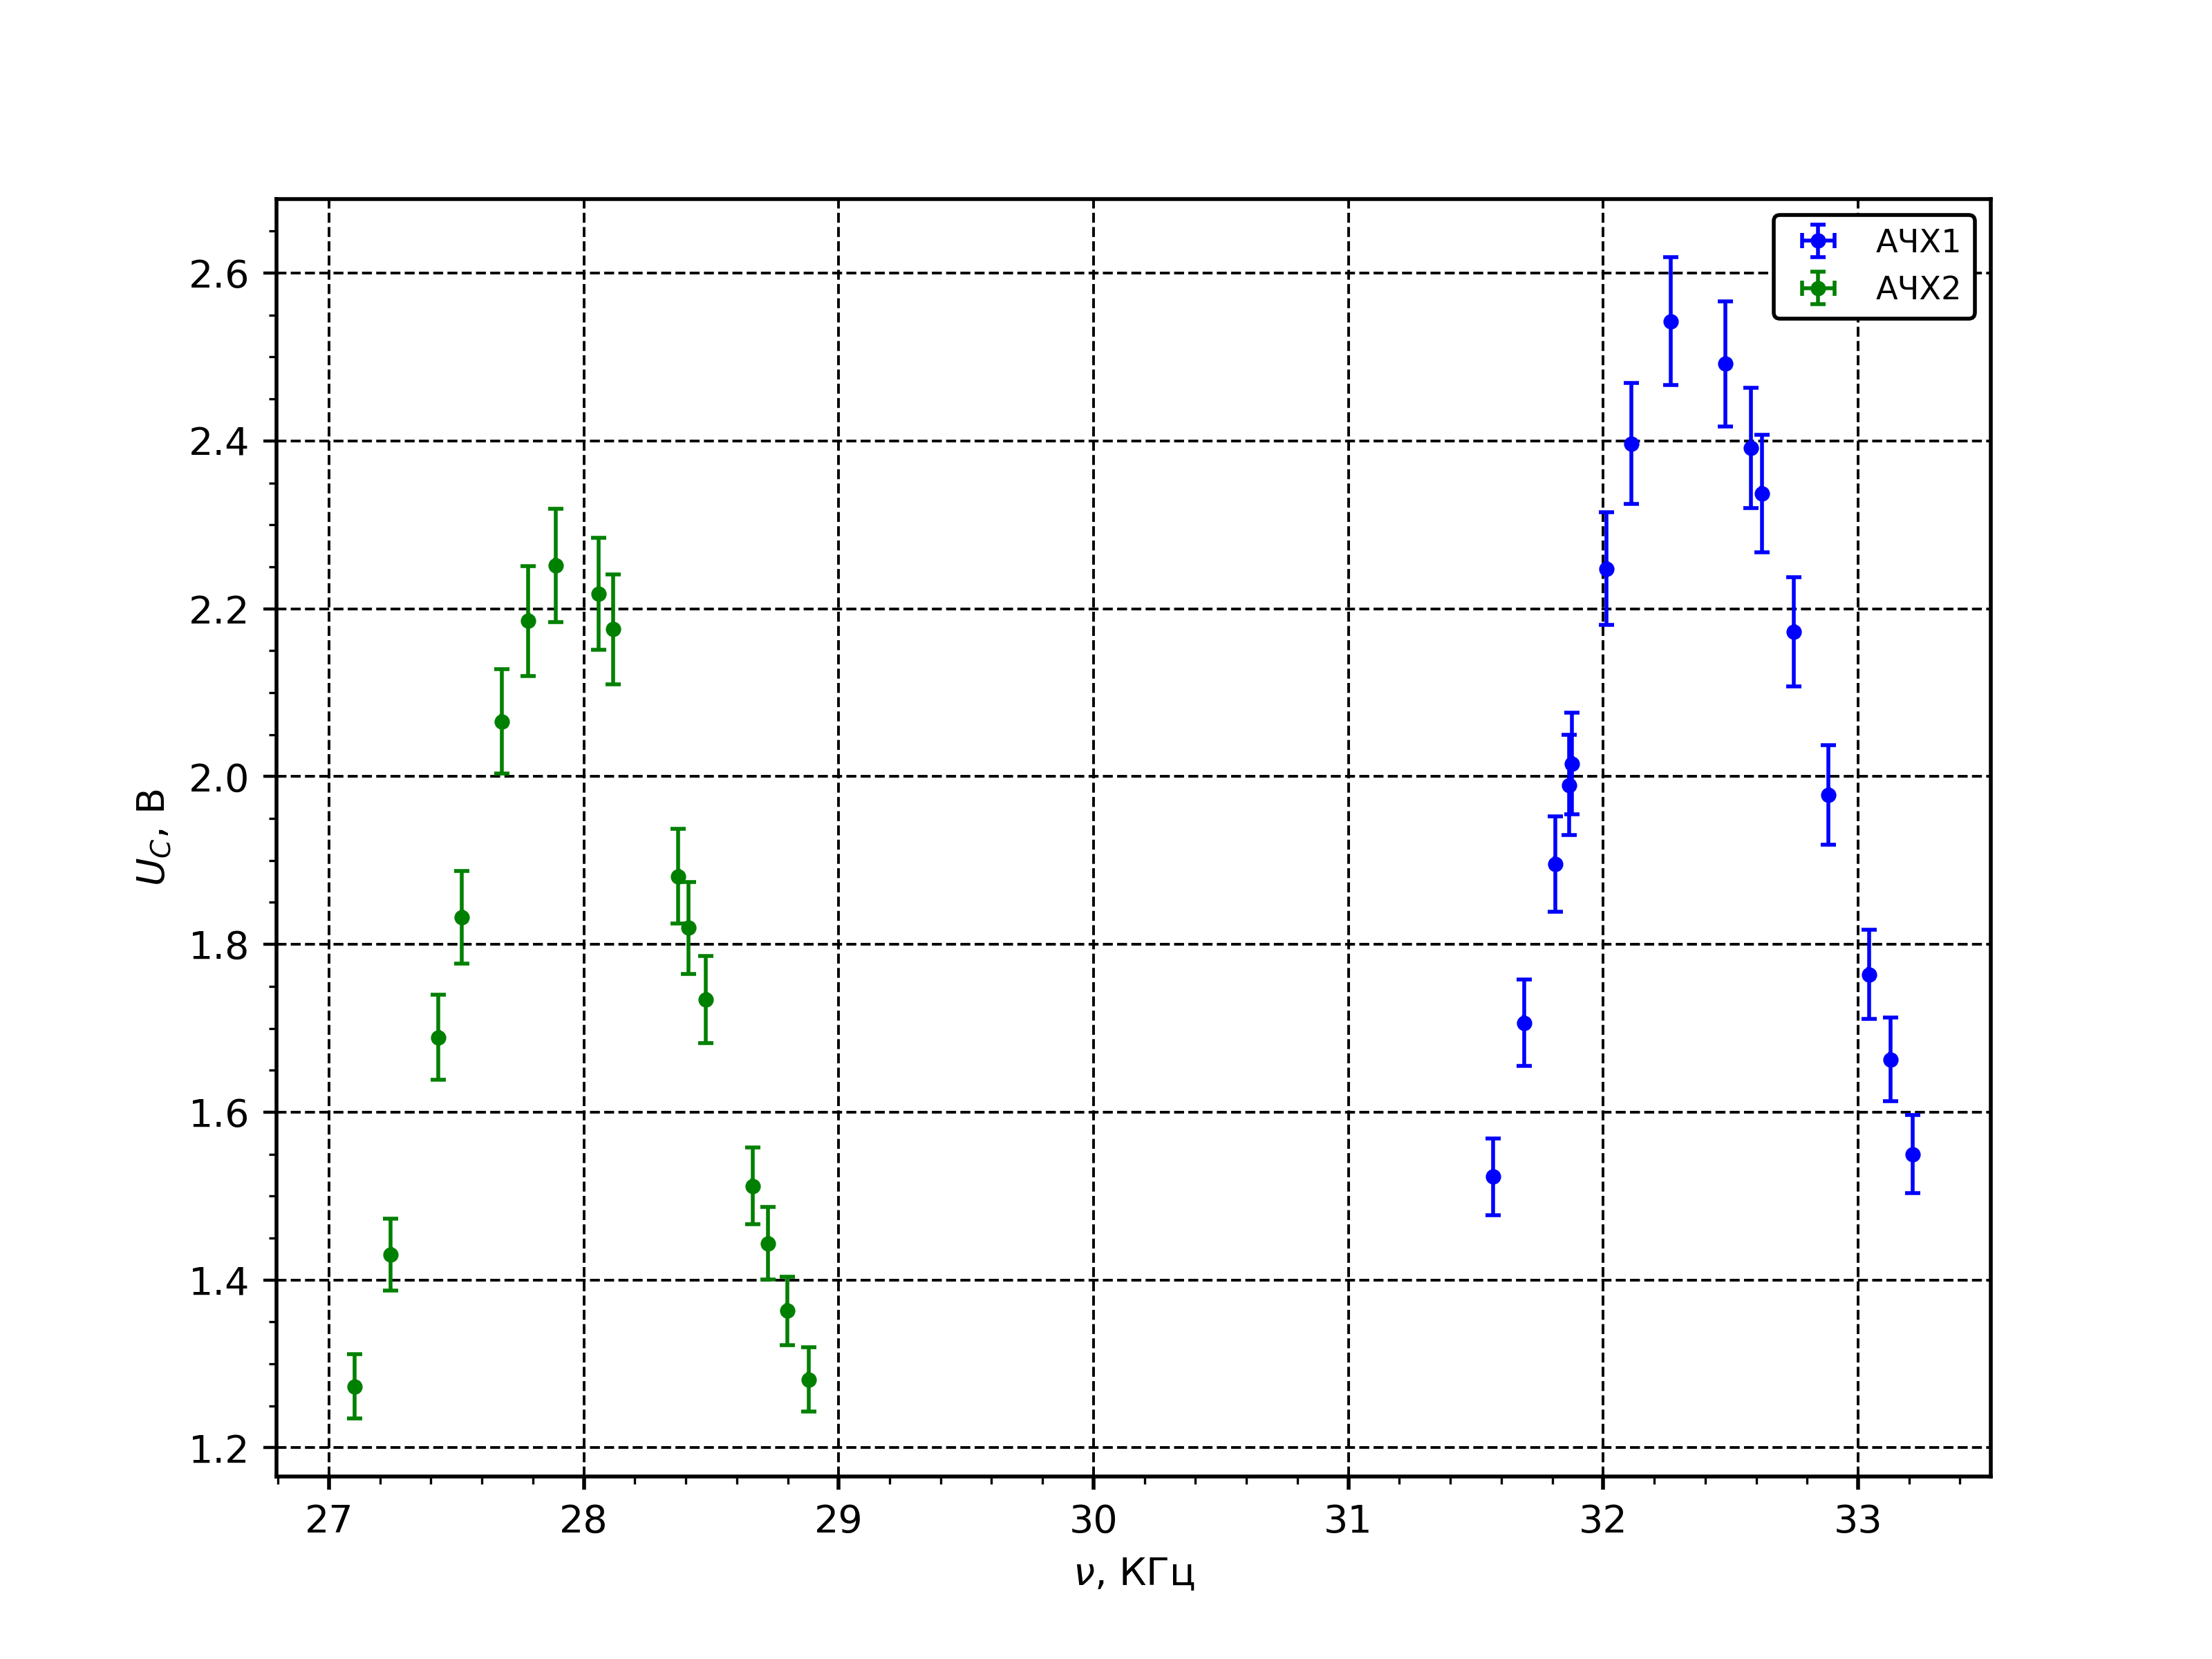
\includegraphics[width=0.8\linewidth]{../img/task9.png}}
\end{figure}

Частоты и напряжения АЧХ1 больше, чем АЧХ2. Из-за того, что напряжения больше, контур 1 добротнее, чем контур 2.

\begin{figure}[ht!]
    \center{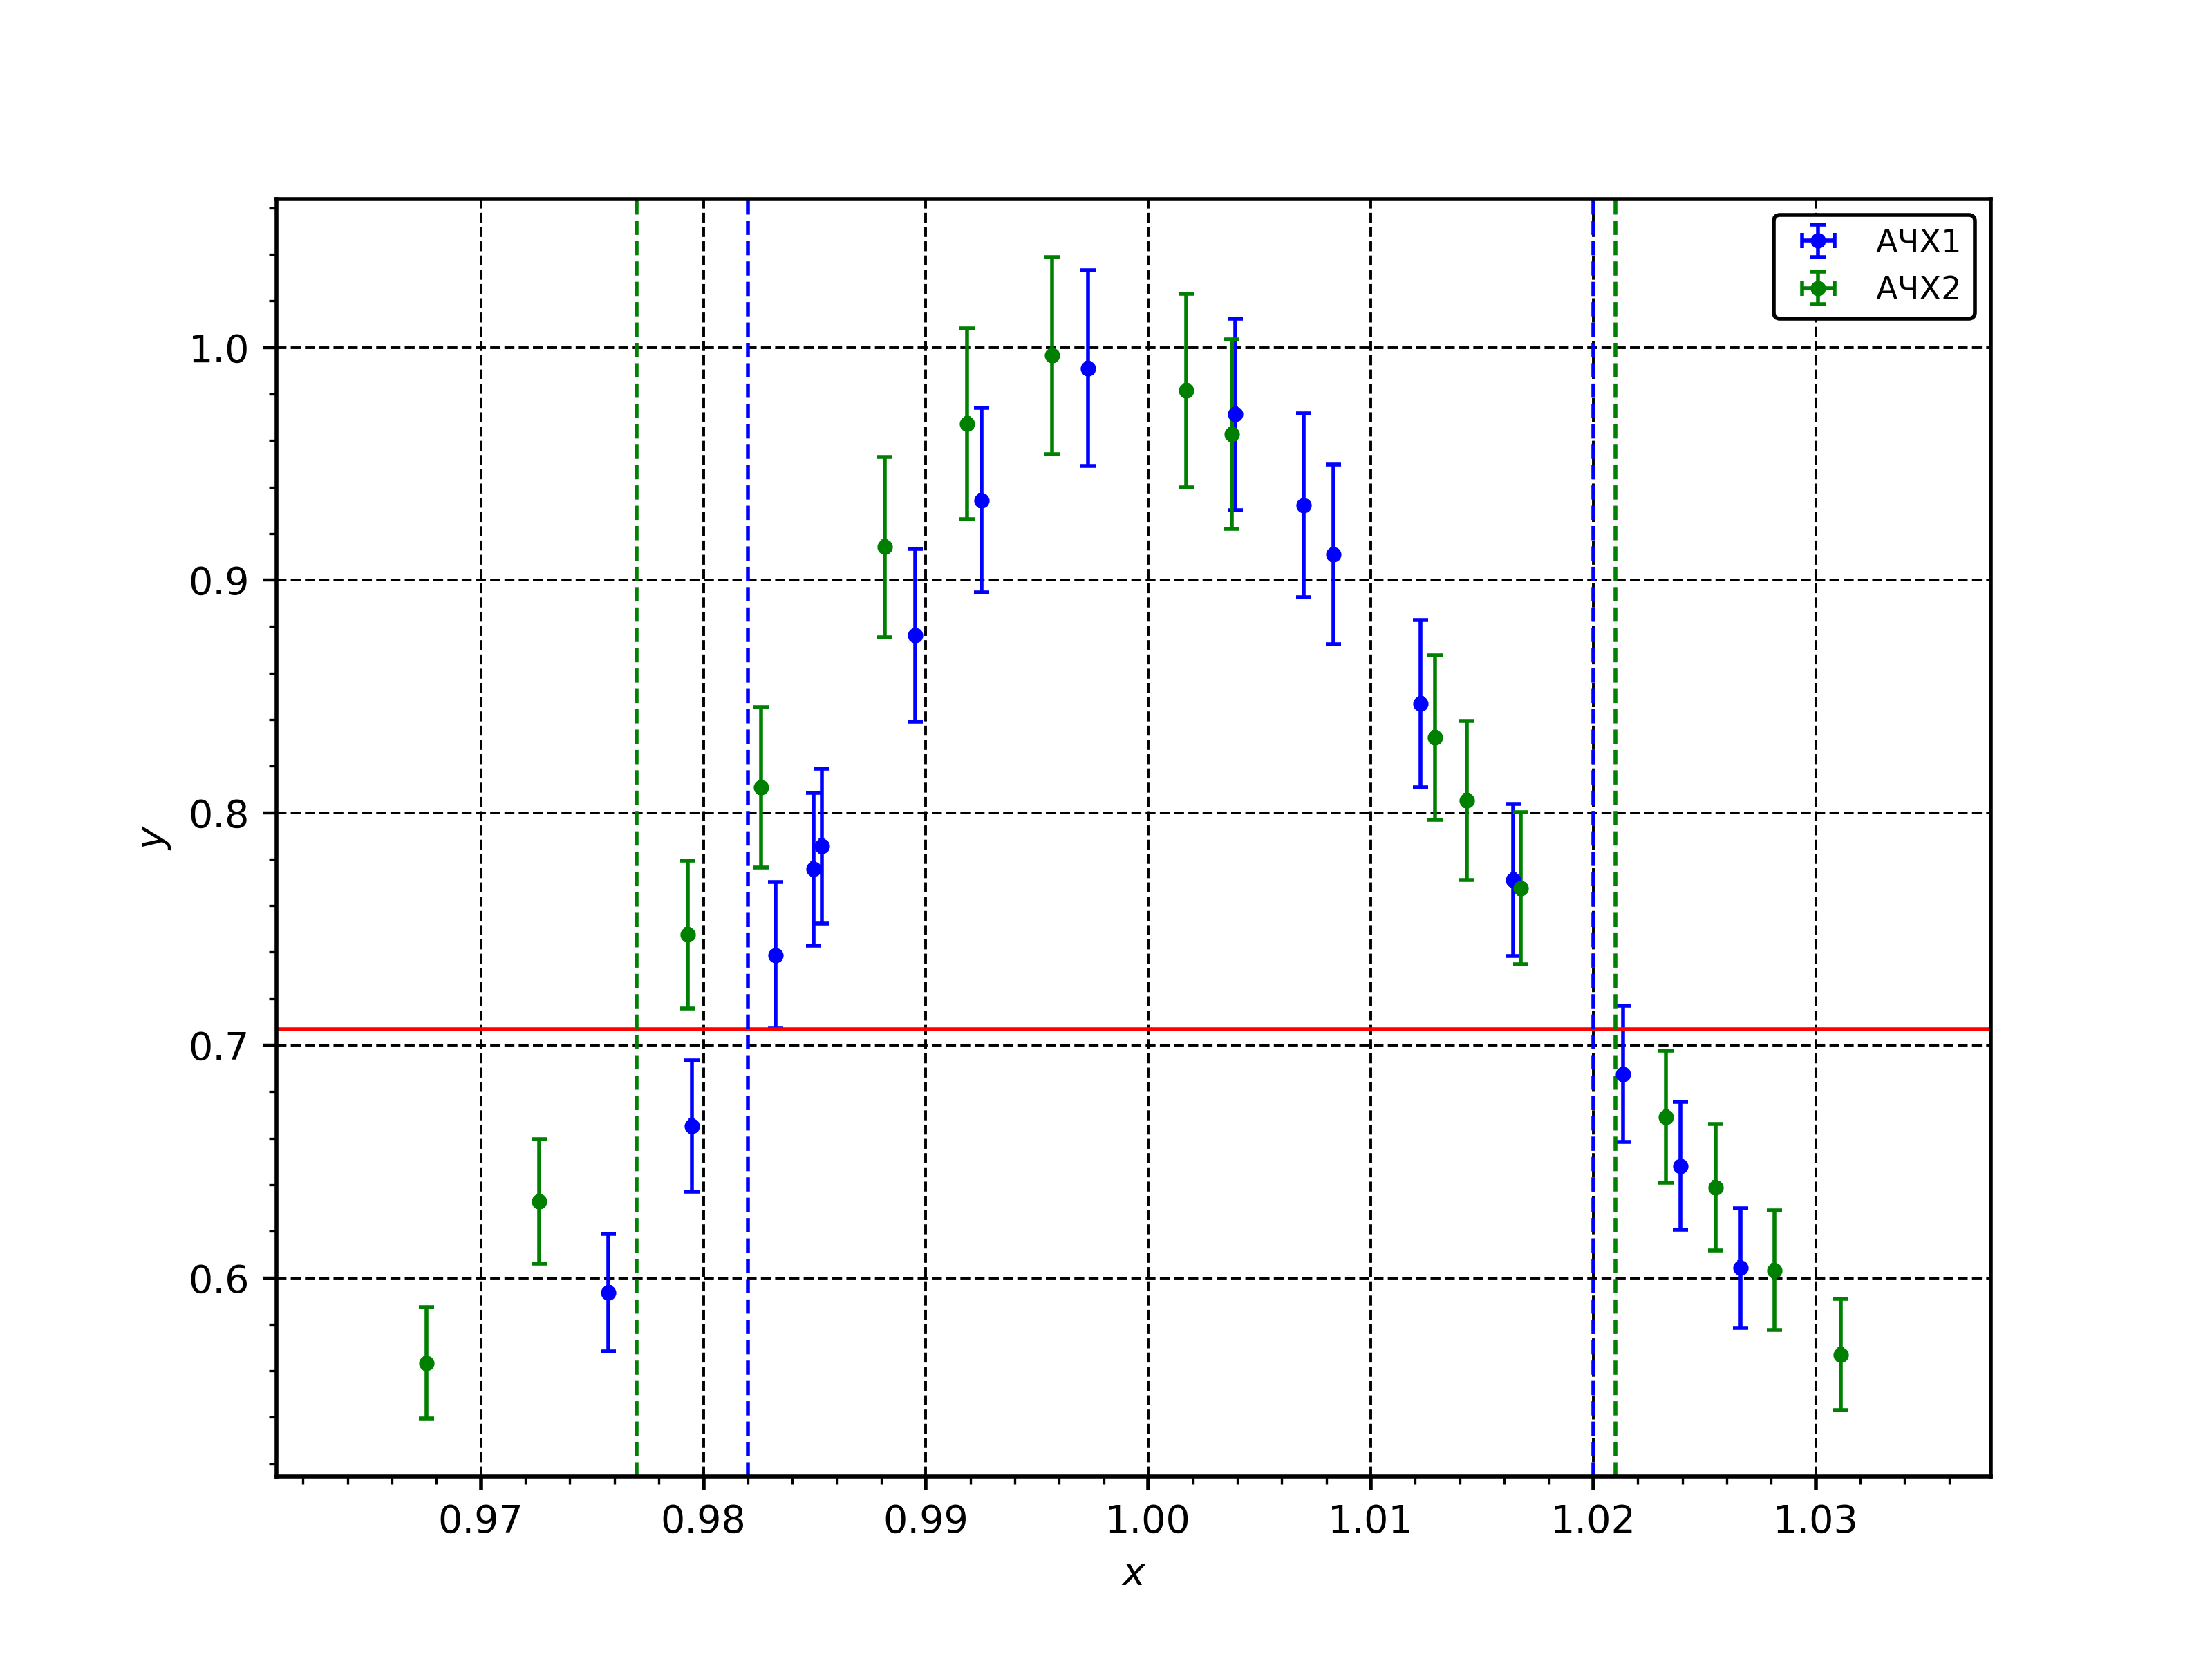
\includegraphics[width=0.8\linewidth]{../img/task10.png}}
\end{figure}

\[
    Q_{1} = \frac{1}{x_{1} - x_{2}} = 26 \pm 2
\]
\[
    Q_{2} = \frac{1}{x_{1} - x_{2}} = 23\pm 2 
\]

\begin{figure}[ht!]
    \center{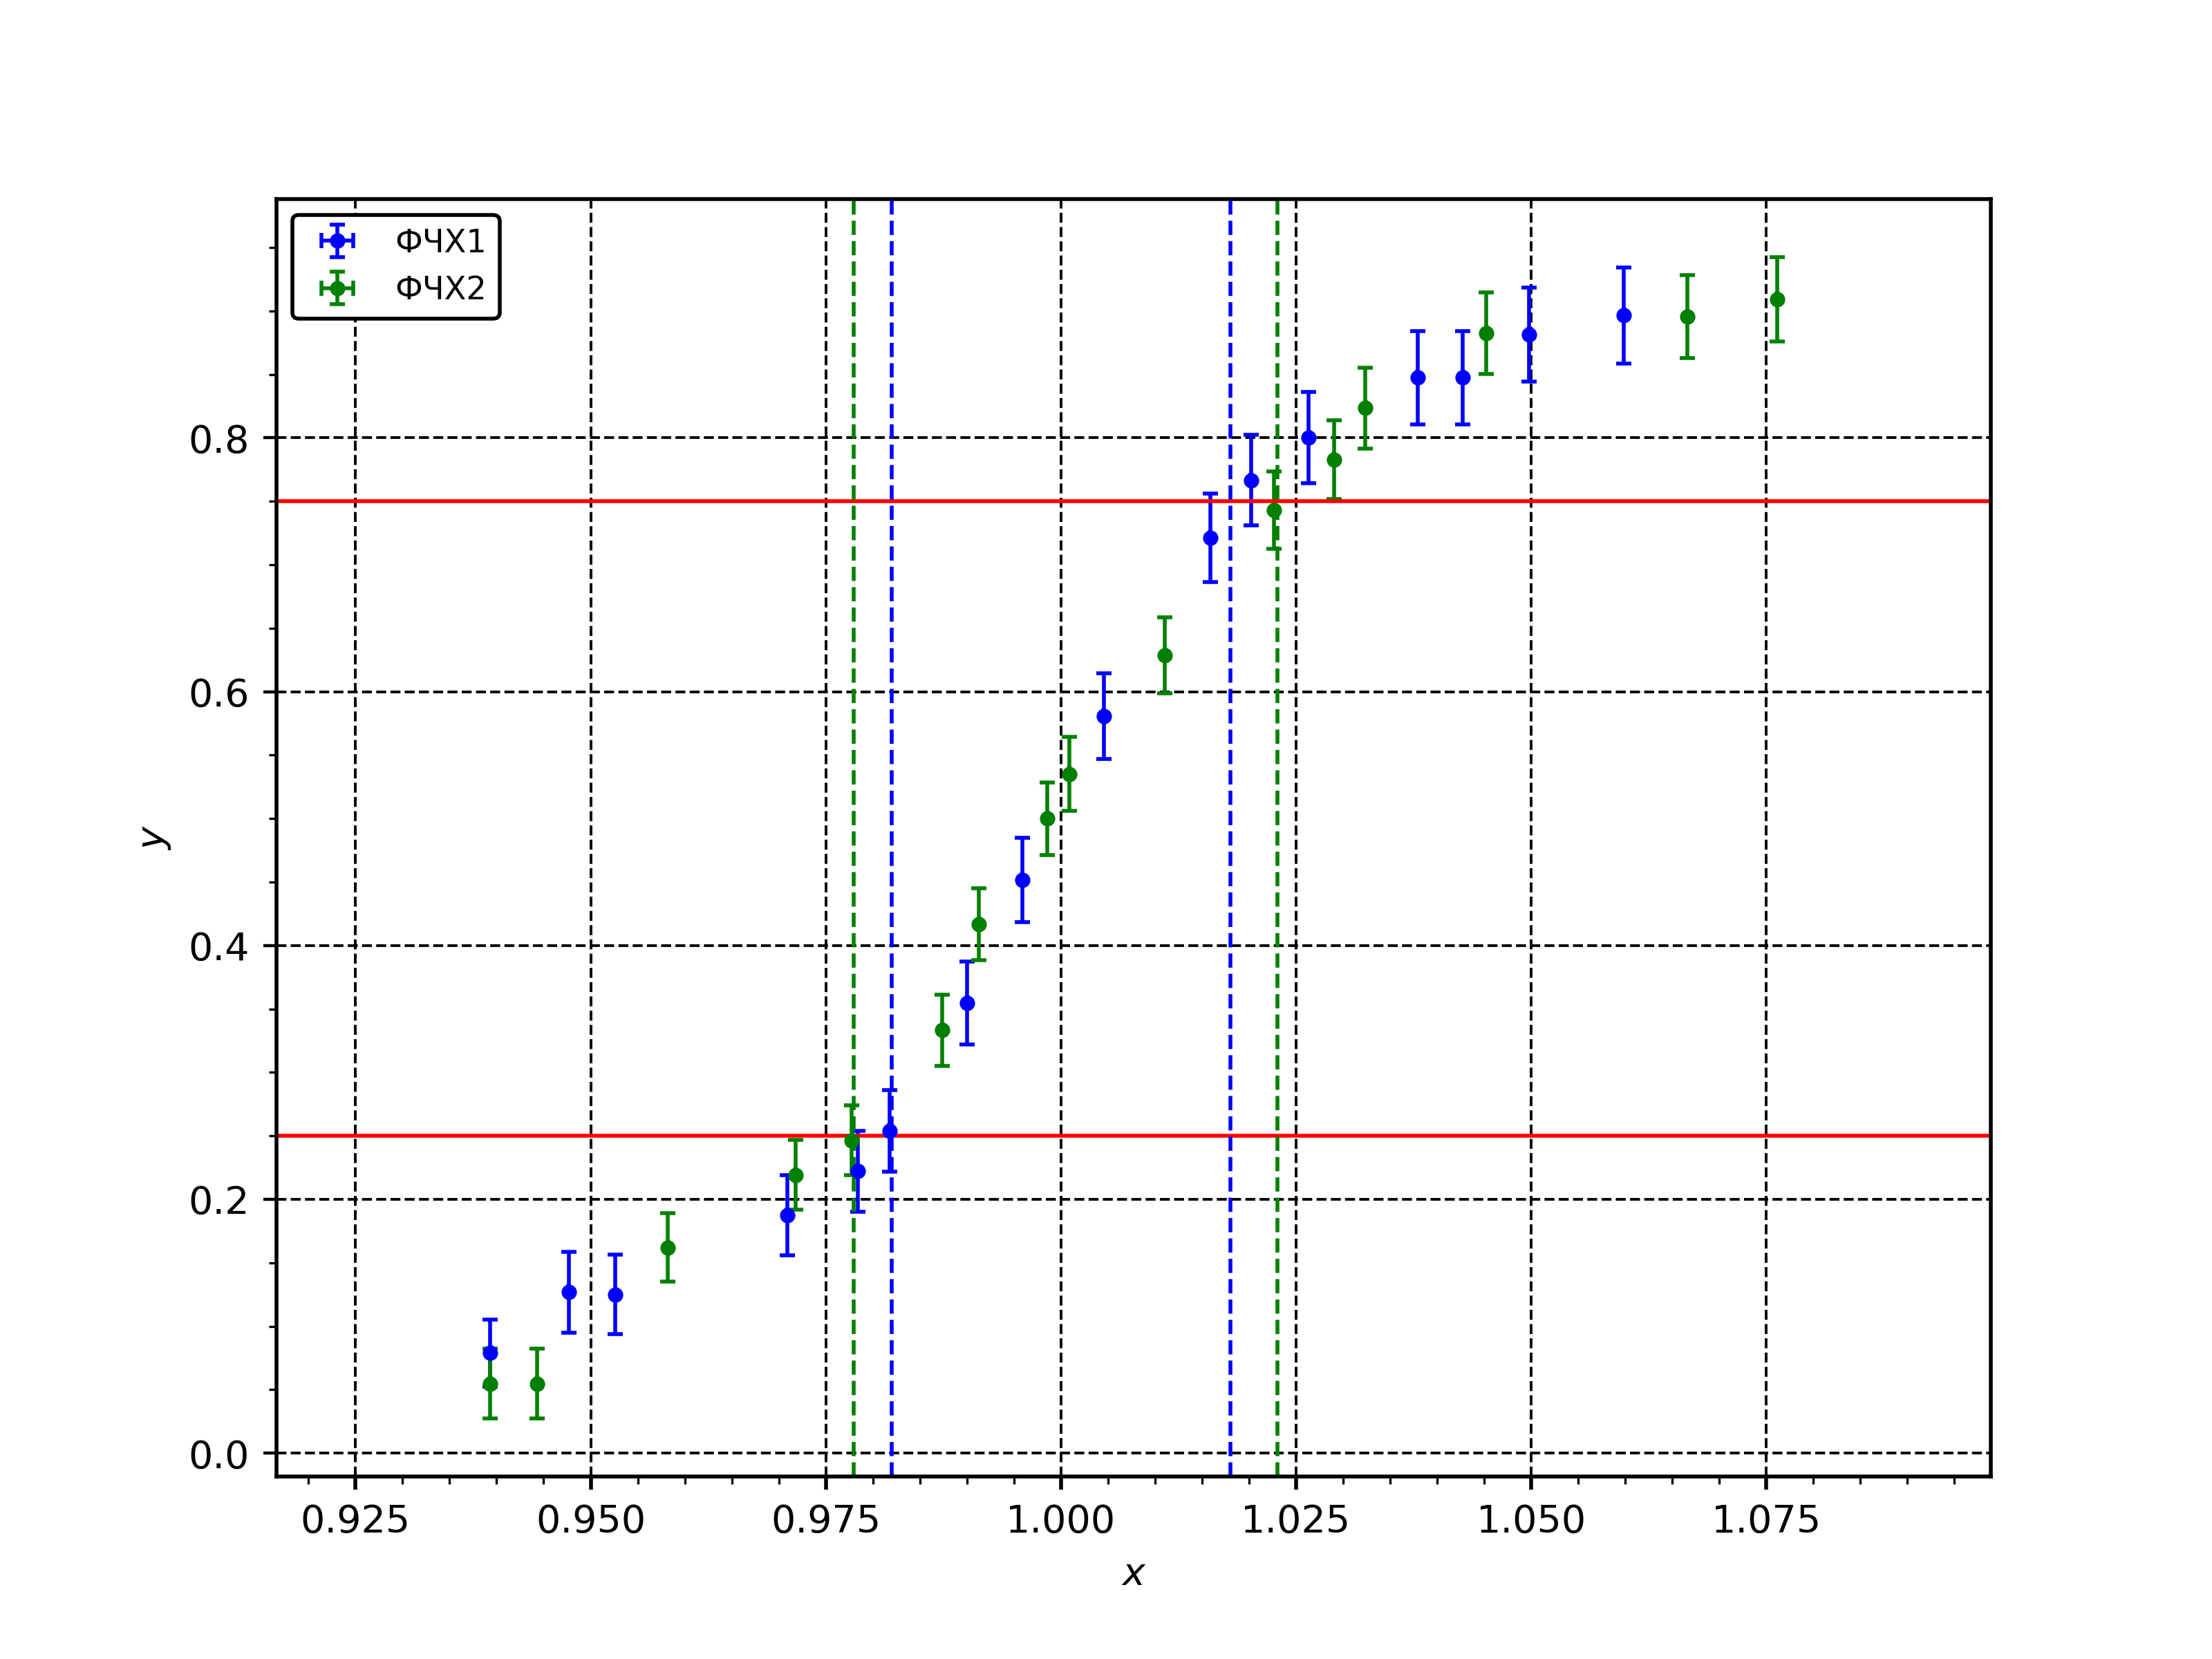
\includegraphics[width=0.8\linewidth]{../img/task11.png}}
\end{figure}

\[
    Q_{1} = \frac{1}{x_{1}-x_{2}} = 28\pm 2
\]
\[
    Q_{2} = \frac{1}{x_{1}-x_{2}} = 22\pm 2
\]

\begin{figure}[ht!]
    \center{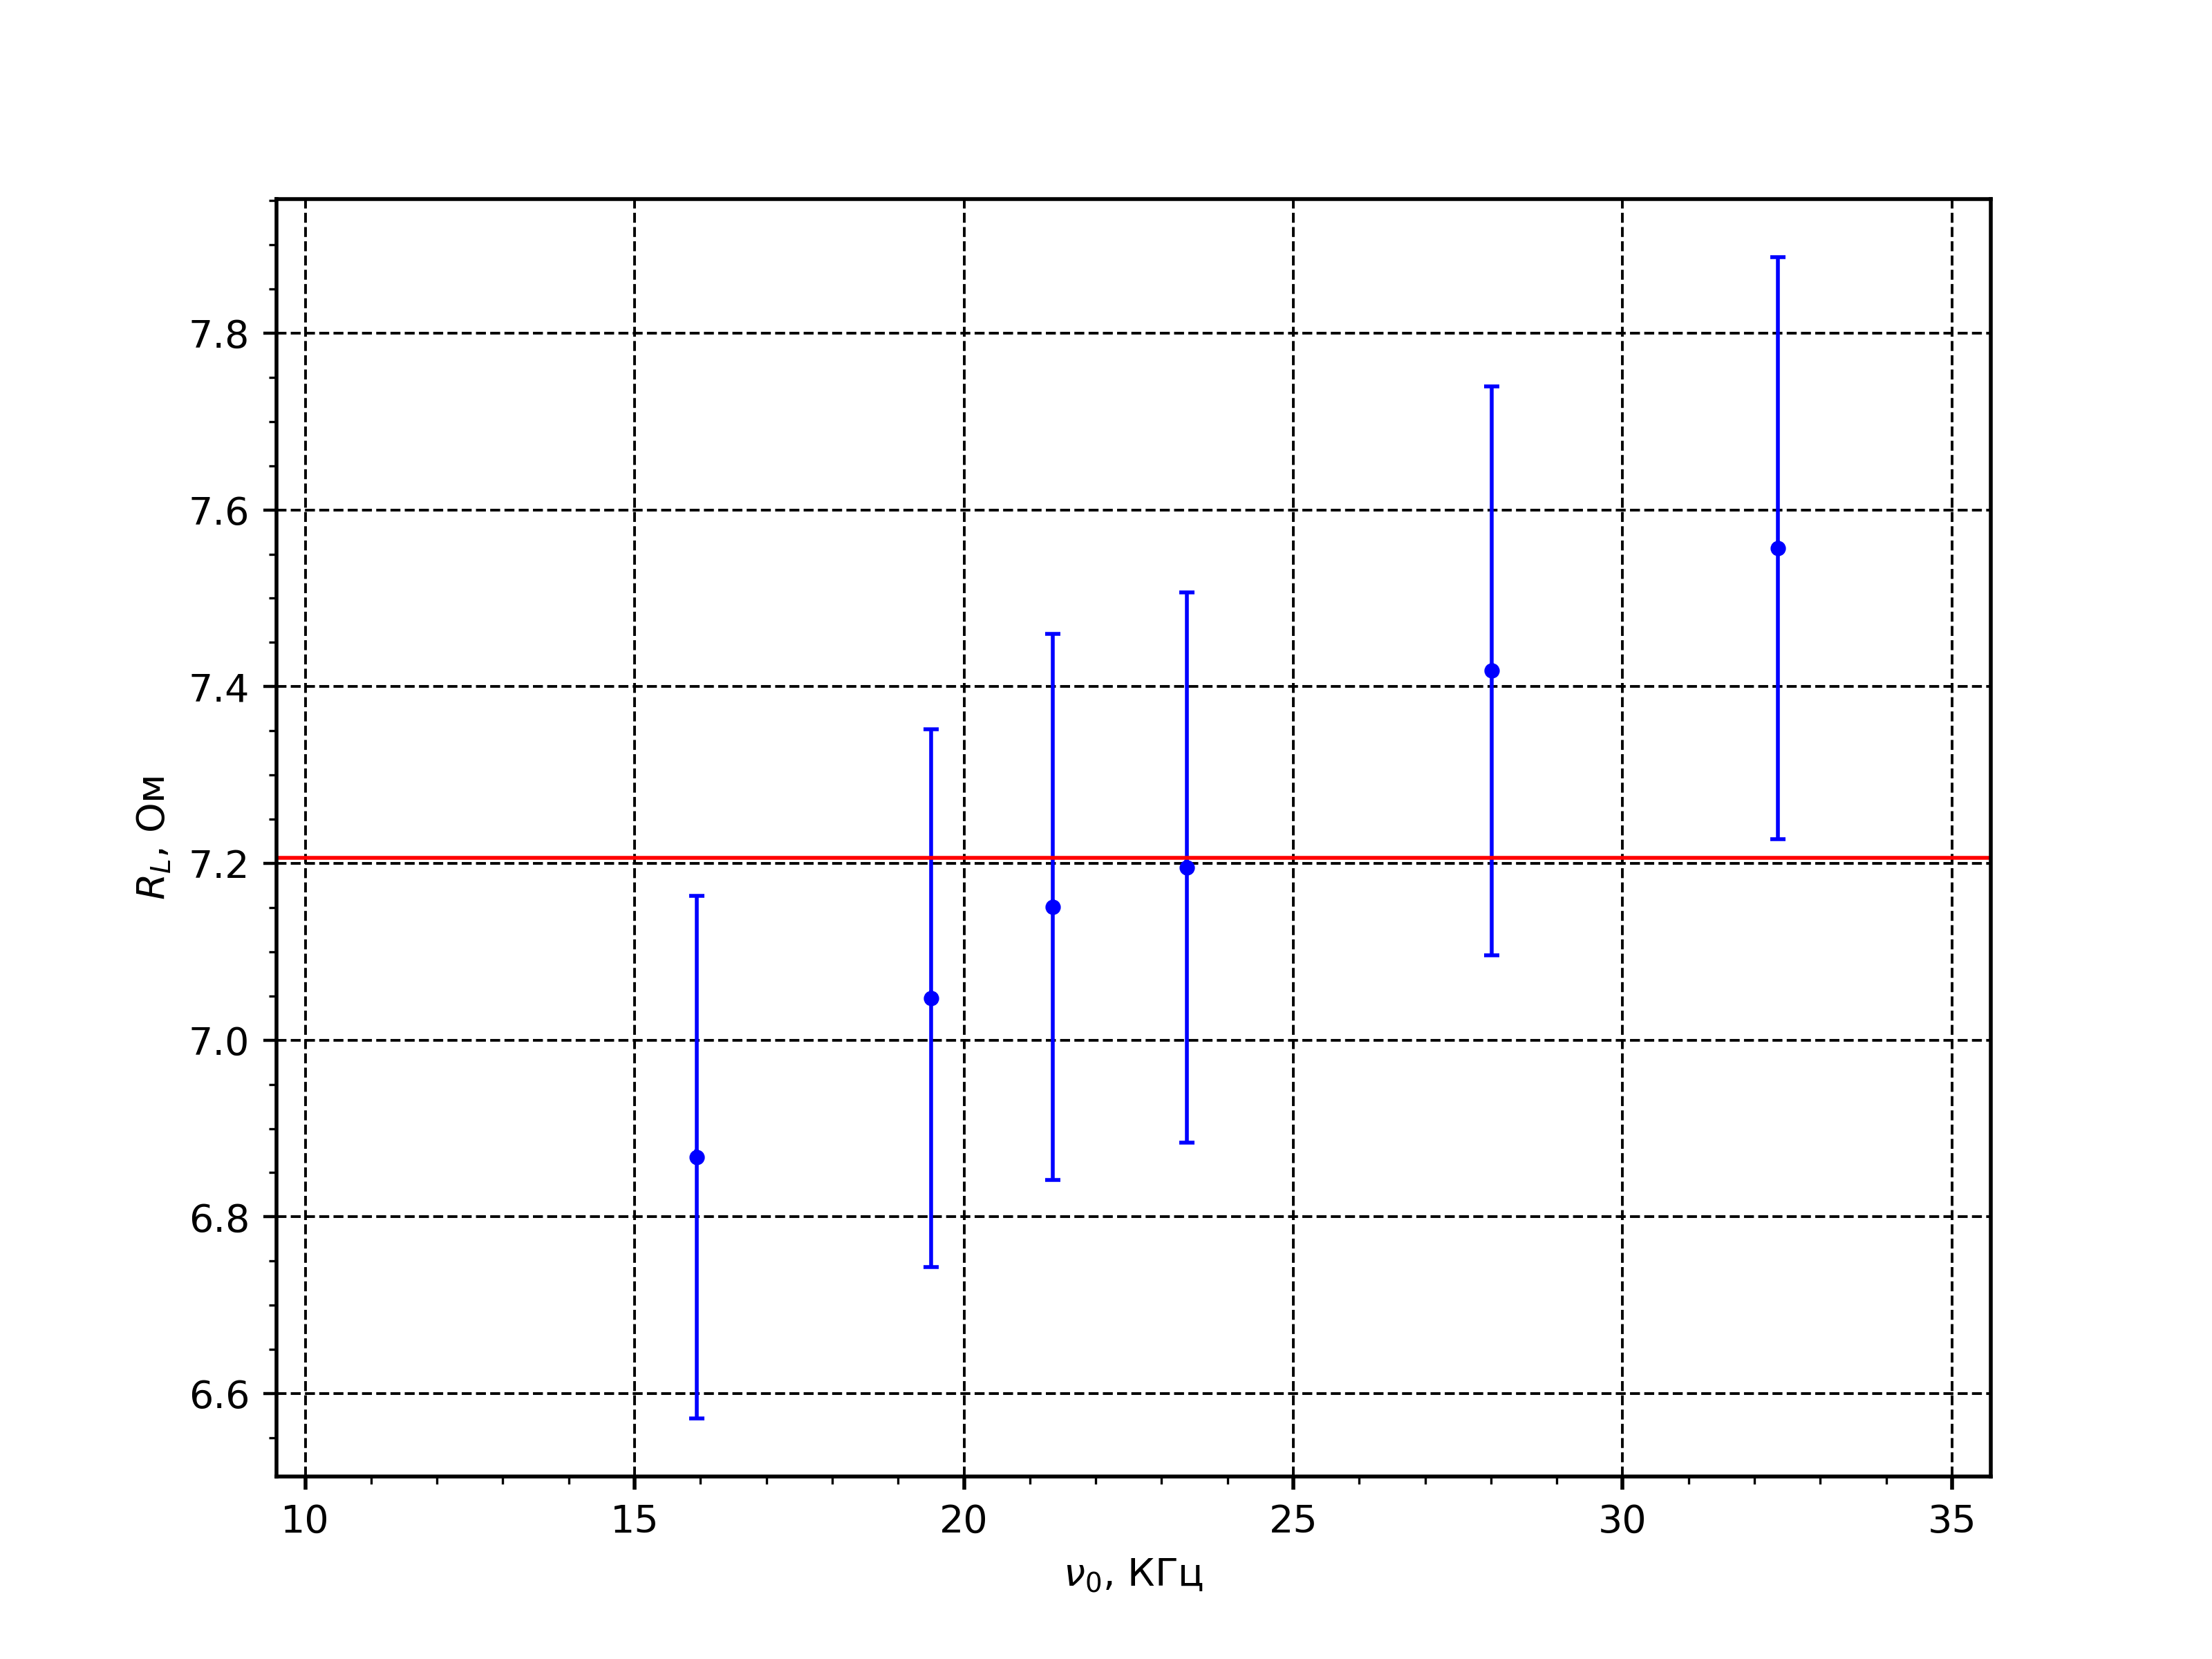
\includegraphics[width=0.8\linewidth]{../img/task12.png}}
\end{figure}

Изменение сопротивления может быть связано с токами Фуко в сердечнике и скин-эффектом.

\begin{figure}[ht!]
    \center{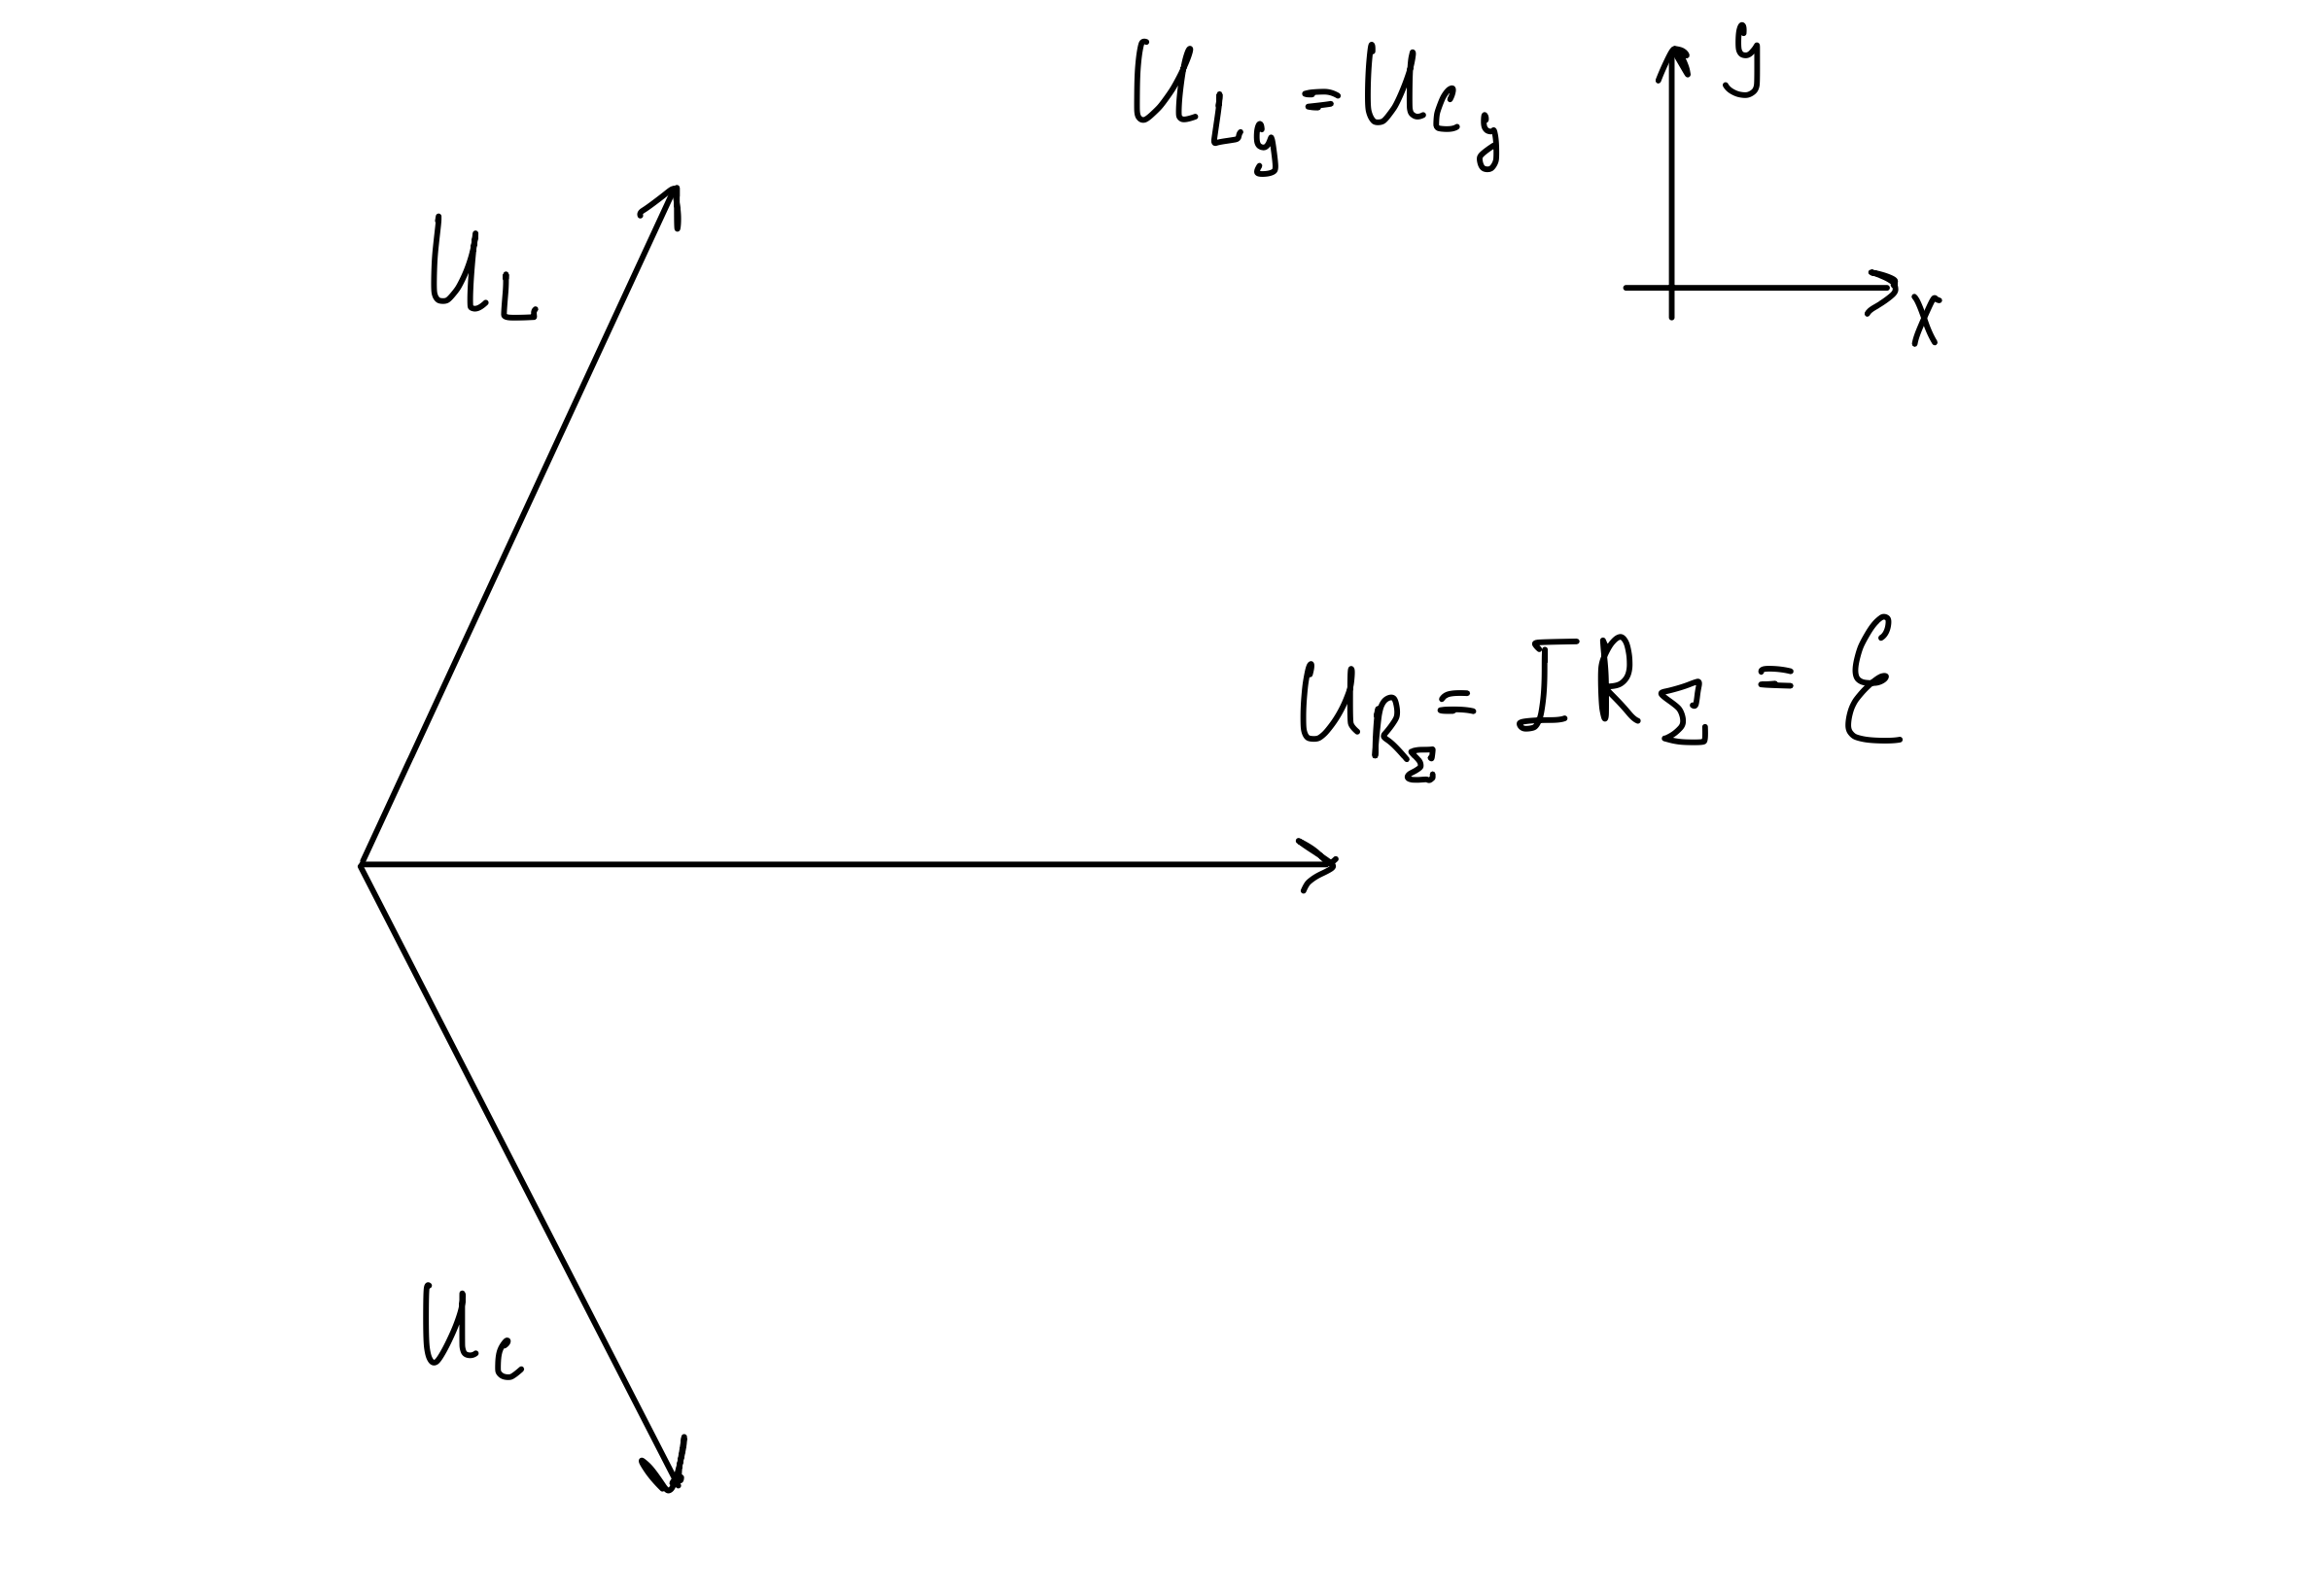
\includegraphics[width=0.8\linewidth]{../img/task13.png}}
\end{figure}

